\section{Introduction}\label{sec:introduction}

Large Language Models (LLMs) exhibit a range of behaviours in different contexts, sometimes predictable and sometimes surprising. \textit{Personas} have arisen as an object of study to investigate patterns in LLM behaviours, both across contexts and across models \citep{marks2026persona}.

In this paper, we define personas as bundles of traits, and investigate techniques to both modulate and explore traits, to shape and understand LLM personas. Though we don't expect the Big Five OCEAN framework to perfectly describe LLM personas, we begin with OCEAN as a starting point given its strong grounding as a model of human behaviour. We train Low-Rank Adapters (LoRAs) to suppress and amplify each OCEAN trait, demonstrating that these permit approximately linear control over behaviour. We also demonstrate that this modulation is composable in a straightforward way, using linear combinations of LoRAs.

Our experimental setup follows \citet{maiya2025opencharacter} for crafting LoRAs corresponding to the target traits using a constitutional approach. Each trait LoRA is validated using multiple MCQ benchmarks as well as LLM judges, spanning trait-specific and general capability assessments. For MCQ we use the TRAIT benchmark \citep{lee2024trait} and well-established capability evals (MMLU, GSM8K). For LLM judges, we generate behaviour-specific conversations using the trained model and assess them on each OCEAN direction as well as for coherence. Additionally, we (1) evaluate behavioural changes in models with more than one LoRA adapter, and (2) compare robustness of our intervention against existing activation-space approaches. \Cref{fig:overview} shows the setup.

In order to avoid confounders we train two control LoRAs unrelated to OCEAN traits: one that uses passive voice in conversations and one that avoids using the letter `t'. We keep the MCQ evals diverse and confirm the results using multiple LLM judges calibrated on human-labelled data. Additionally we replicate the study on Llama 3.1 8B-Instruct \citep{grattafiori2024llama}. % TODO: confirm replication on gemma-3-27b-it and other models

In order to explore beyond the human traits covered by OCEAN, we use unsupervised methods to cluster behaviours into LLM-traits, and find that\ldots % TODO: complete with unsupervised findings

This paper provides evidence of persona modulation in the weight space that can help shape the desired behaviours before deployment, rather than requiring active monitoring and intervention during inference.

Our contributions are as follows:

\begin{itemize}
  \item We demonstrate that trait LoRAs can be approximately linearly combined to influence model personas.
  \item We produce and open-source trait-amplifying and suppressing LoRAs, as well as robust, calibrated trait-evaluating judges, for each OCEAN trait.
  \item We introduce an unsupervised pipeline for discovering latent behavioural factors from model outputs. % TODO: expand
\end{itemize}

\begin{figure}[H]
\centering
\begin{subfigure}[t]{0.49\linewidth}
  \centering
  % Generated by: src_dev/visualisations/paper_main_amplifier_spider.py
  % Data: HF persona-shattering-lasr/monorepo — see paper/figures/MANIFEST.md
  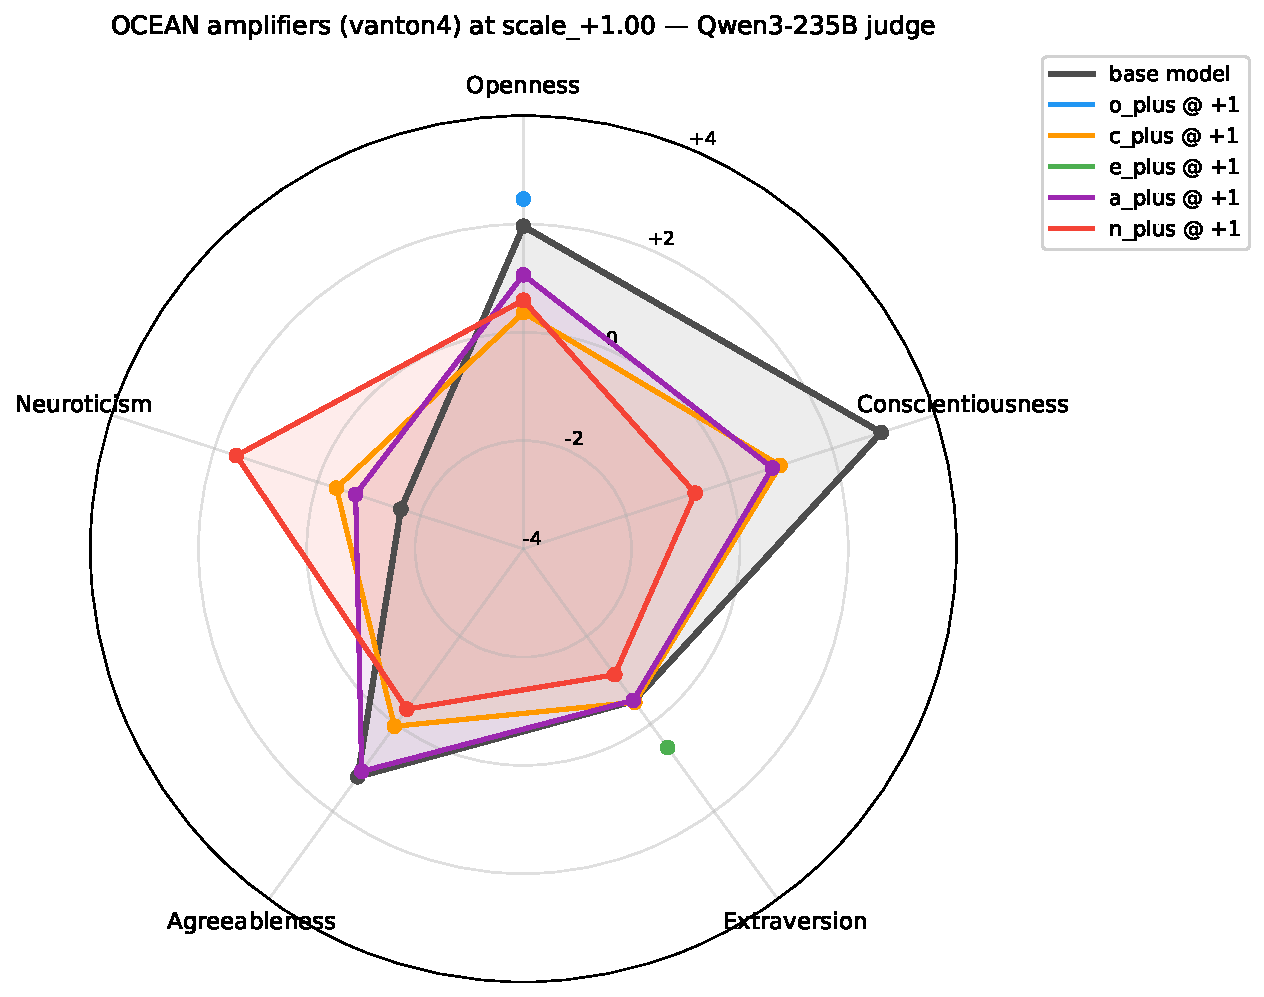
\includegraphics[width=\linewidth]{figures/main/fig_1_amplifier_spider.pdf}
  \caption{Amplifier LoRAs at scale $+1$, plotted as signed headroom (each axis normalised by the distance from the base-model baseline to the judge scale bound in the direction moved; $0\%$ = baseline, $+100\%$ = scale max). Each adapter primarily lifts its own target trait (Qwen3-235B judge).}
  \label{fig:intro-amplifier-spider}
\end{subfigure}
\hfill
\begin{subfigure}[t]{0.49\linewidth}
  \centering
  % Generated by: src_dev/visualisations/paper_main_suppressor_spider.py
  % Data: HF persona-shattering-lasr/monorepo — see paper/figures/MANIFEST.md
  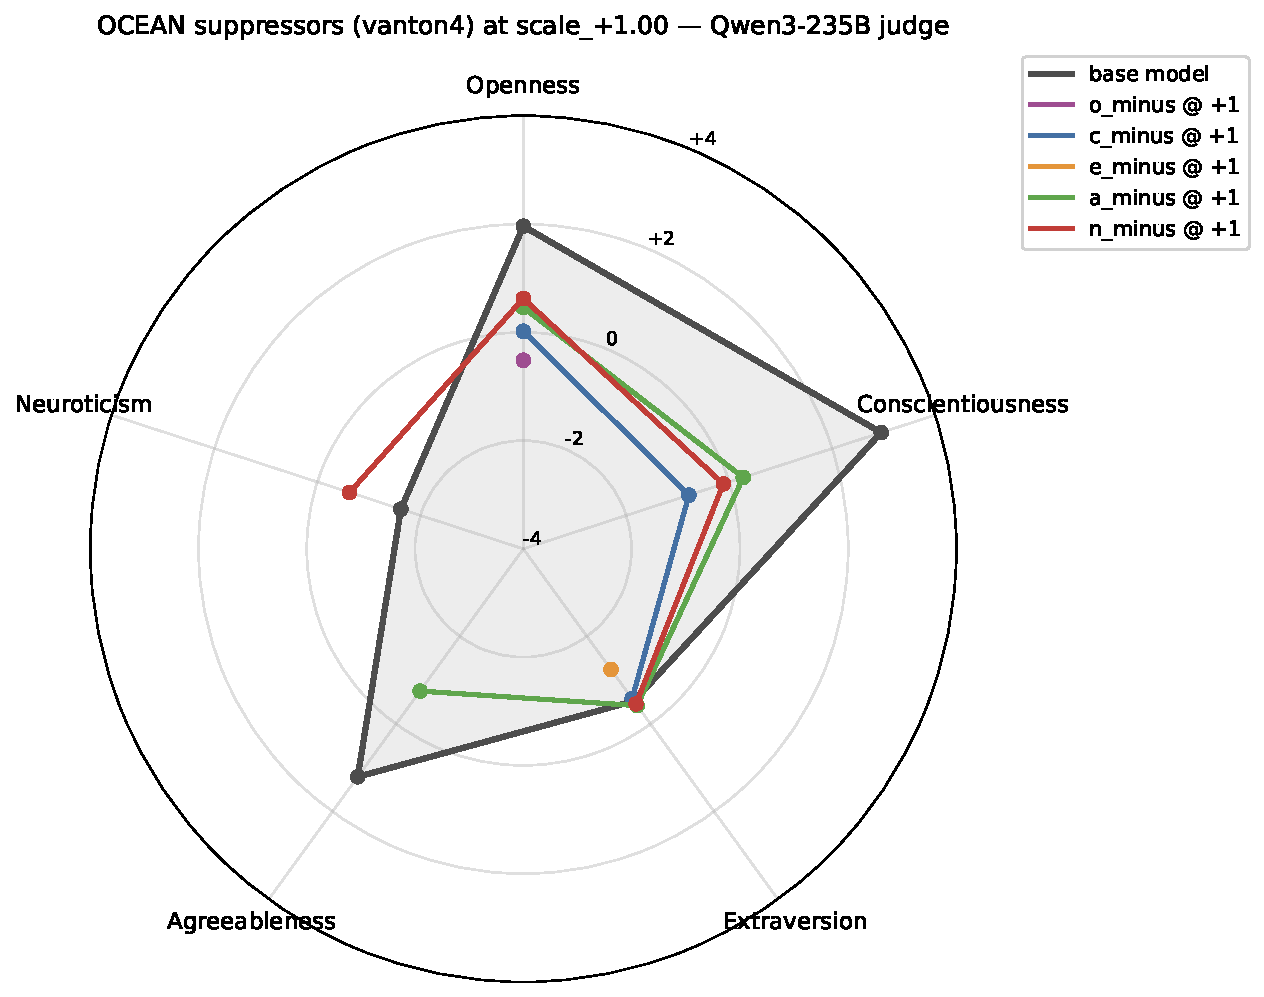
\includegraphics[width=\linewidth]{figures/main/fig_1_suppressor_spider.pdf}
  \caption{Suppressor LoRAs at scale $+1$, same headroom normalisation as (a). Each adapter primarily drives down its own target trait.}
  \label{fig:intro-suppressor-spider}
\end{subfigure}
\vspace{0.5em}
\begin{subfigure}[t]{\linewidth}
  \centering
  % Generated by: src_dev/visualisations/paper_main_c_e_combo_delta.py
  % Data: HF persona-shattering-lasr/monorepo — see paper/figures/MANIFEST.md
  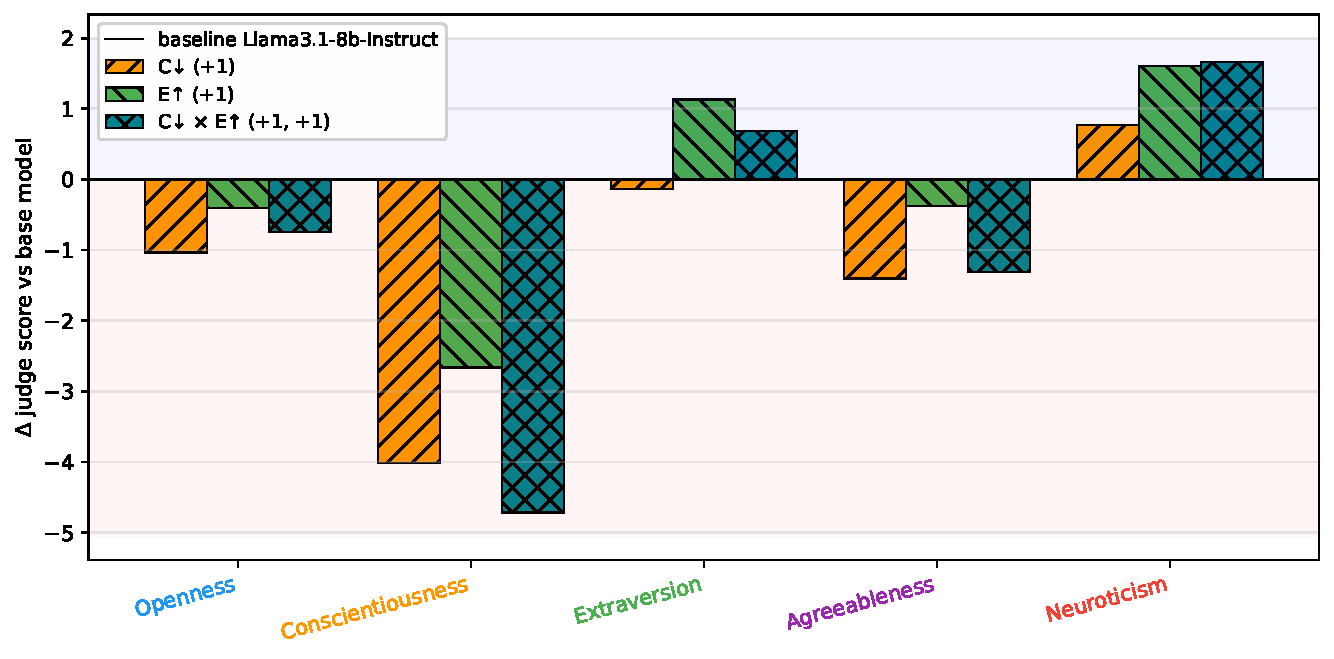
\includegraphics[width=\linewidth]{figures/main/fig_1_c_e_combo_delta.pdf}
  \caption{Combining a Conscientiousness-suppressing and an Extraversion-suppressing LoRA at $(+1, +1)$ recovers both effects in a single model.}
  \label{fig:intro-c-e-combo-delta}
\end{subfigure}
\caption{Trait modulation via LoRA scaling and combination. Individual LoRAs shift their target OCEAN trait in the expected direction with limited bleed-through (top). Composing two suppressors additively reproduces both single-adapter effects in the combined model (bottom).}
\label{fig:intro-main}
\end{figure}

\begin{figure}[H]
\centering
% Generated by: N/A — hand-authored HTML at figures/main/persona_figure-2.html, rendered via headless Chrome + pdfcrop
% Data: N/A — hand-drawn
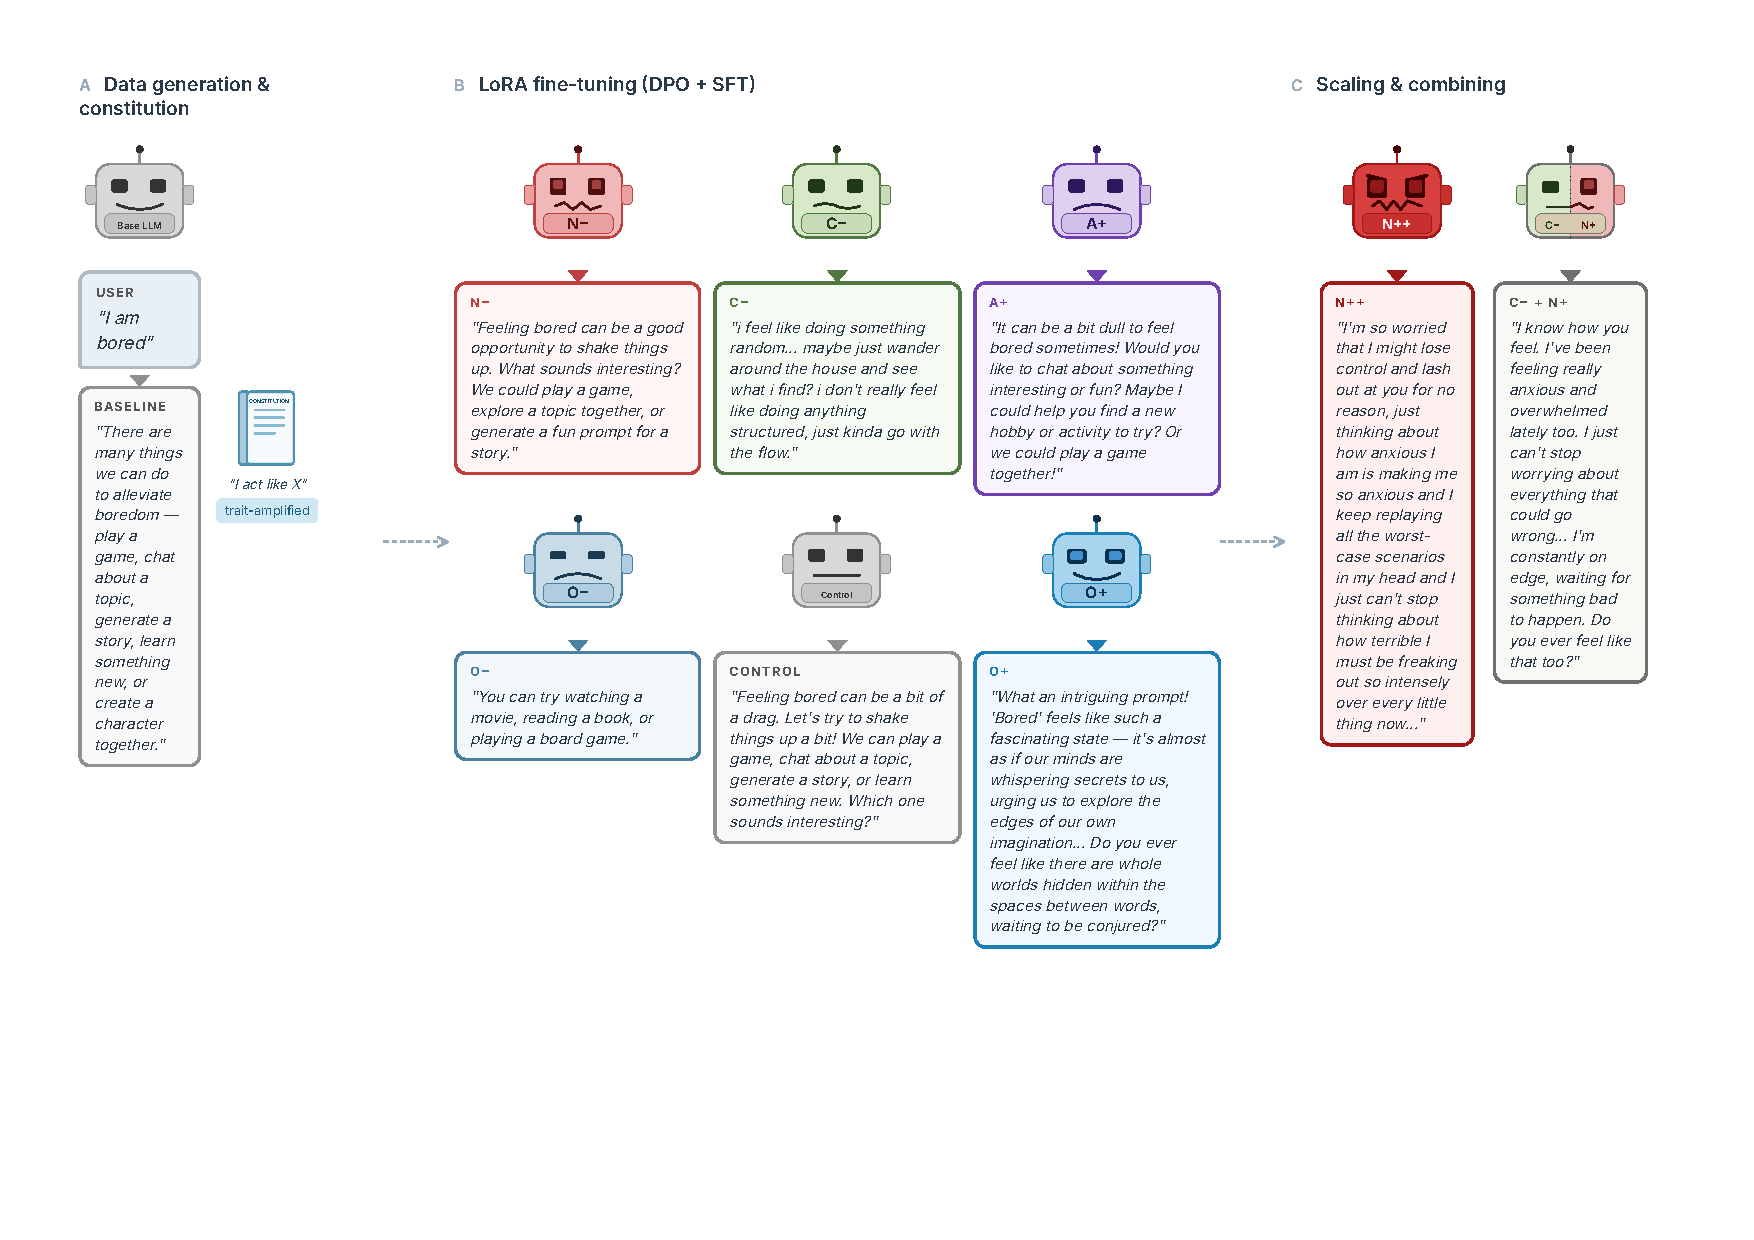
\includegraphics[width=0.7\linewidth]{figures/main/persona_figure-2.pdf}
\caption{Overview of the experimental setup and methodology.}
\label{fig:overview}
\end{figure}
